\section{Introduction}

Cartons have been widely used in the packaging industry to organize, ship, and deliver various commodities, which include food, daily necessities, and electronic components. 
Beyond the very basic packaging shapes like cuboids, extremely elaborate packaging exists for certain specialty items, such as wedding candies or wine bottles. 
The popularity of such intricate designs has increased, not to mention the fact that they are environmental friendly due to their recycalbility and degradability~\cite{Mullineux:2010:CSC:1739328.1739673}.

Cartons are usually designed based on experience and trial-and-error.
Designers typically start a package design by generating 2D vector artwork; then, a 3D mockup is essential for designers and clients to see the real appearance~\cite{guide}. There are two ways to create a 3D mockup.
A digital mockup is a great, inexpensive way of showing how the design would appear in real life, plus it allows designers to repeatedly modify the layout.
%A digital mockup is a great way of showing how the design would appear with lower cost and is convenient for designers to modify the layout repeatedly. 
A physical mockup is also helpful when making sure the size is correct in order to make a final decision. 
%
Due to the low cost and efficiency of digital mockups, there have been many software packages developed to help designers improve their design efficiency and productivity.
%
For example, the commercial software named STUDIO~\cite{STUDIO} generates 3D models by manually assigning angles to folding edges. 
By using models, users can turn their ideas into beautiful 3D images.
Moreover, it is non-trivial for non-expert users to figure out how to fold a complex carton using only a 2D crease pattern. A digital simulation system would provide valuable references to inspire creativity~\cite{Thiel1998,Kishi:1998:OFP:786112.786279,Nimnual2007Virtual}. 
However, the existing softwares still requires extensive manual skill to design cartons.
%Researchers have also studied in obtaining 2D layouts from unfolding 3D objects for decades. However, the unfolded layouts are fragile in some parts which are not suitable for fabrication~\cite{Tai2004Unfolding} and sometimes are not feasible to fold.
In order to create a virtual 3D model and explore diverse layouts, our idea is to fold the existing layout directly into a 3D model, and reach a variety of layouts by manipulating the corresponding model.


It is nontrivial to mathematically formulate the problem of model construction using only a planar layout, because the information extracted from the 2D pattern, such as edge length and vertex degree, may cause ambiguities on account of repeated edges and vertexes. 
Moreover, Biedl et al.~\cite{Biedl:2005:NFP:1090462.1646553} proved that given a polygon and a set of creases, it is NP-hard to know whether a polyhedron can be obtained by folding along the creases, which can also illustrate the difficulty of our problem.

\begin{figure}
	\centering
	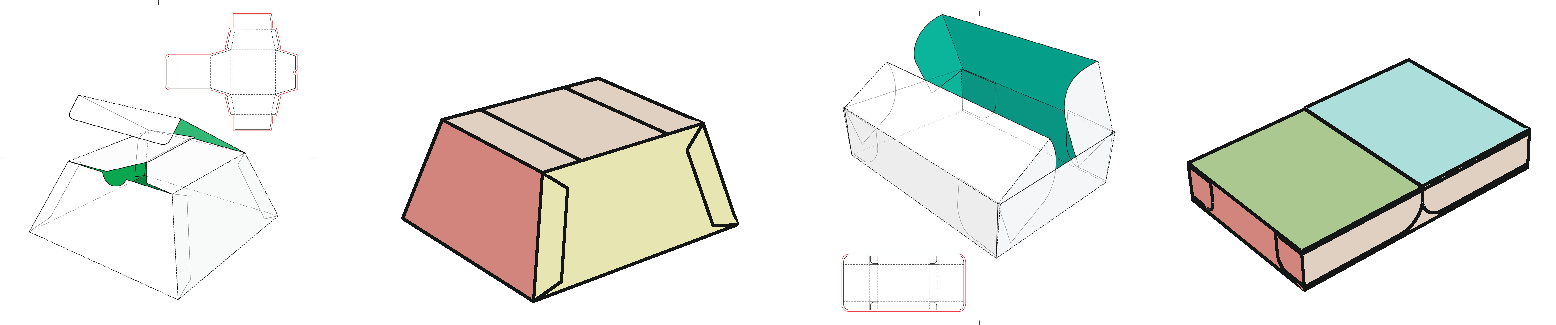
\includegraphics[width=0.9\textwidth]{images/artist}
	\caption{Two cartons and artist-designed layouts. The corresponding 3D models are folded according to our system.}
	\label{fig:artist}
\end{figure}

 
 
In order to solve the folding cartons using 2D layouts as our only input, we present an optimization method when given a set of shape constraints.
Moreover, an interactive design and exploration framework is proposed to allow users to visualize planar layouts and corresponding models in a 3D view and freely edit the models. 
The original layout can be corrected and explored by optimization. Figure~\ref{fig:artist} shows our folding results based on a series of 2D layouts designed by artists. 

The contributions of this paper includes the following:

(1) An interactive and explorative system to manipulate the shapes of 3D cartons. Our system creates corresponding models using rough initializations and user interactions. Imprecise layouts can be modified with a geometric optimization. Users may easily edit these 3D models in order to explore alternative deformed layouts
%3D model by a rough initialization and user interactions, and modifies imprecise layouts by a geometric optimization. Users are allowed to edit the 3D model to explore deformed layouts automatically.

(2) A collection of shape constraints, which are represented through a set of points, are used to implement shape optimization. Based on observations of existing cartons, constraints are summarized by including panel rigidity and coplanarity to maintain the integrity of the cartons' shapes. 
In addition, computer-aided detection, like vertex merging and panel pasting, is introduced to offer suggestions to users. 